\documentclass[11pt,a4paper]{scrartcl}
\usepackage[T1]{fontenc}
\usepackage[utf8]{inputenc}
\usepackage[ngerman]{babel}
\usepackage{microtype}
\usepackage{lmodern}
\usepackage{amsmath}
\usepackage{amsfonts}
\usepackage{amssymb}
\usepackage{enumerate}
\usepackage{csquotes}
\usepackage{graphicx}
\usepackage{hyperref}

\begin{document}

\author{Gruppe 14\\Max-Emanuel Hoffmann\\Ralf Vogler\\Sebastian Wiesner}
\title{Verteilte und Web-Informationssysteme}
\subtitle{Blatt 11}

\maketitle

\section{RDF and SPARQL}

\begin{enumerate}

\item[1)] Welche Wissenschaftler, die in Hamburg geboren wurden, haben einen Nobelpreis gewonnen?\\
\begin{verbatim}
select ?x where {
  ?x <bornInLocation> "Hamburg".
  ?x <hasWonPrize> "Nobel_Prize".
  ?x <type> "wordnet_scientist_110560637"
}
<Gustav_Ludwig_Hertz>
<James_Franck>
\end{verbatim}


\item[2)] Welche Firmen wurden in Silicon Valley im Jahr 2004 gegründet?\\
\begin{verbatim}
select ?x where {
  ?x <establishedOnDate> "2004".
  ?x <type> "wordnet_company_108058098".
  ?x <locatedIn> "Silicon_Valley"
}
No entries
\end{verbatim}
online: <Namesys> \footnote{\href{''https://d5gate.ag5.mpi-sb.mpg.de/webyagospotlx/WebInterface?passedQuery=I%3A1%09S%3A\u003fc%09P%3Atype%09O%3Acompany%09LP%3Anearby%09LV%3ASilicon%20Valley%3BI%3A0%09S%3A\u003fx%09P%3Acreated%09O%3A\u003fc%09TP%3Aduring%09TV%3A2004%3B
''}{''YAGO 2 spotlx''}}
\begin{verbatim}
select ?x where {
  ?x <establishedOnDate> "2004".
  ?x <type> "wordnet_company_108058098".
  ?x <locatedIn> "California"
}
<TextDrive>
\end{verbatim}


\item[3)] Mit wem ist Steven Spielberg verheiratet?\\
\begin{verbatim}
select ?x where { ?x <isMarriedTo> "Steven_Spielberg" }
<Amy_Irving>
<Kate_Capshaw>
\end{verbatim}


\item[4)] In welchen Filmen hat Adam Sandler mitgespielt?\\
\begin{verbatim}
select ?o where { <Adam_Sandler> <actedIn> ?o }
"Anger_Management"
"Big_Daddy_(film)"
\end{verbatim}

\end{enumerate}


\section{RDF-3X}
\subsubsection*{Geben Sie das resultierende Dictionary und die komprimierten Blätter des SPO-Index an!}
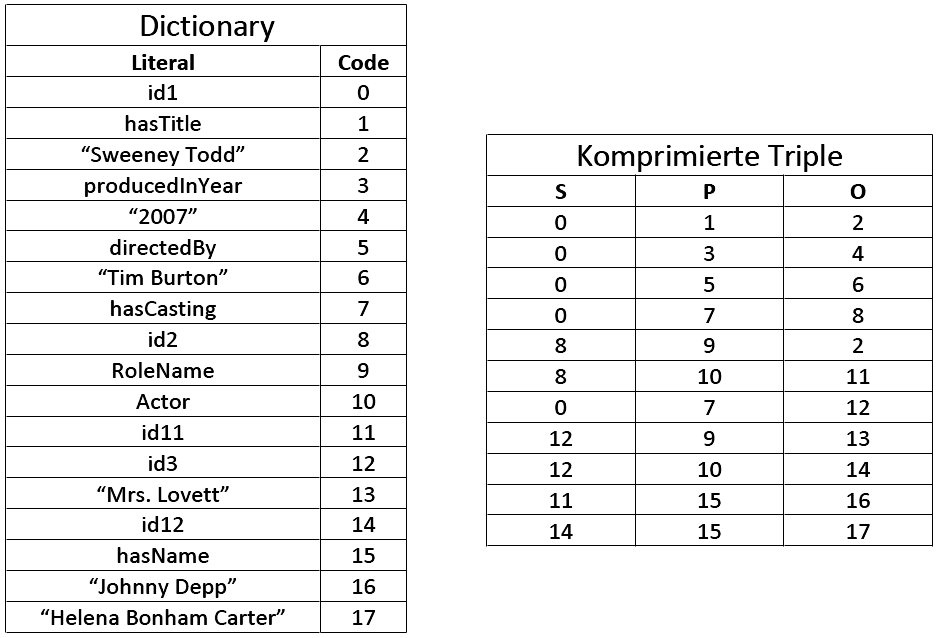
\includegraphics[width=\textwidth]{triple.png}
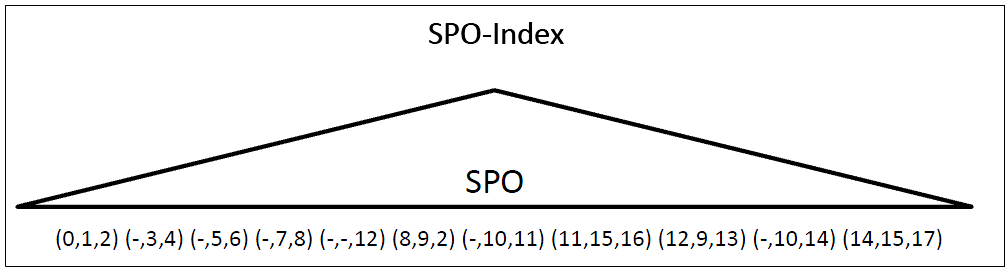
\includegraphics[width=\textwidth]{baum.png}
In einem Blatt wird eigentlich nur der Unterschied zum vorherigen Blatt gespeichert. Dies wurde der Einfachheit halber weggelassen.

\subsubsection*{Was berechnet die Anfrage?}
\begin{verbatim}
select ?n where {
  ?p <hasName> ?n . ?s <Actor> ?p.
  ?s <RoleName> "Sweeney Todd"
}
\end{verbatim}
Gibt die Namen der Schauspieler aus, die die Rolle des Sweeney Todd gespielt haben.

\subsubsection*{Geben Sie den Ausführungsplan in RDF-3X an und erläutern Sie ihn.}
% PO (<RoleName> "Sweeney Todd"), SP (?s <Actor>), SP (?p <hasName>)
\begin{enumerate}
\item Literale im Query werden über B+-Baum durch ihre IDs ersetzt.\\
Es ergibt sich:
\begin{verbatim}
select ?n where {
  ?p 15 ?n. ?s 10 ?p. ?s 9 2
}
\end{verbatim}
\item Im Folgenden werden die Pattern über den SPO-Index oder Permutationen davon gesucht (Die Variablen müssen dabei ein Suffix sein). Gibt es mehrere Möglichkeiten für einen Index, wird derjenige gewählt, der wahrscheinlich die höhere Selektivität am Anfang erreicht.\\
Mögliche Abfolge:\\
\begin{enumerate}
\item ?s 9 2 -> OPS
\item ?s 10 ?p -> PSO
\item Danach wird ein Merge-Join über die Subjekte der beiden Ergebnismengen durchgeführt, da beide sortiert vorliegen.
\item ?p 15 ?n -> PSO
\item Hash-Join (weil Kandidaten nicht sortiert) von Objekt ?p (?s 10 ?p) und Subjekt ?p (?p 15 ?n).
\item Projektion auf den Namen ?n und umwandeln der IDs in Literale über eine direktes Mapping -> Ergebnis "Johnny Depp".
\end{enumerate}
\end{enumerate}

\end{document}
